\documentclass[a4paper]{article}

\usepackage[english]{babel}
\usepackage[utf8]{inputenc}
\usepackage{amsmath}
\usepackage{enumitem}
\usepackage[T1]{fontenc}
\usepackage{graphicx}
\usepackage{amsmath,amsfonts,amssymb}
\usepackage[colorinlistoftodos]{todonotes}
\usepackage{float}

\title{ECE 498 - Homework 2}

\author{Amod Agrawal, amodka2}

\date{\today}

\begin{document}
\maketitle

\hfill \newline
\textbf{Problem 1}\\ 
\newline \hfill

a. False\\
The DFT of a signal may not symmetric about F\textsubscript{s}/2 if the signal is not real. \\

b. True\\
To solve the localization linear equation, it is essential to synchronize the clocks on the satellite and the receiver because it uses ToF estimates. The time drift between the clocks is modeled as another variable in the GPS equation and is solved for. The clock is synchronized to that value.\\

c. False\\
Signal is attenuated by the environment and therefore, signal strength may not be a good measure for distance. For example, if the AP is very close to us but right across a thick metal wall - the signal strength may still be very low as it gets attenuated \& reflected by the wall.\\

d. True\\
More the number of access points we have, we capture more dimensions at each spatial point. This makes it a higher dimensional space and reduces the ambiguity while doing kNN. Of course, accuracy is also a function of density of war-driving.  \\

e. True\\
For a static object, the accelerometer values are not polluted by linear acceleration. Therefore, both gravity and magnetic north can be used as anchors to find the orientation of the object. Note that the magnetometer readings remain unpolluted by motion of the device, however, may be polluted by magnetic fluctuation in the environment.  \\

f. False\\
If the transmitter is in near field, the assumption of parallel source rays fails and it's not possible to find angle of arrival.  \\

g. False\\
It is important for the time-of-flight measurement to be accurate as well because phase wraps at 2$\pi$. It's not possible to know how many $\lambda$ times has the signal traveled to recollect at the receiver with phase $\phi$.\\

h. True\\
Accelerometers the force acting on the device, that is, when we are holing the phone in our hands - we are actively putting a force of \textit{g} on it against the gravity. In the case of free fall, no force is acting on the device in the local reference frame of the device.\\

i. False\\
The accelerometer data needs to be projected on to the GRF using the orientation estimate -- the resulting projection is then double integrated to find the location estimate. Even if the white noise mean is zero, we're not just summing it up. We are projecting erroneous data based on an erroneous estimate and then double integrating it (which leads to exponential accumulation).\\

j. False\\
Rotation is not commutative because every rotation can only be decomposed to one set of rotation matrices in order (along x, y, and z axes). Yaw, Pitch and Roll rotation matrices actually change the eigenspace of the matrices and therefore, they are not commutative.\\

k. True\\
Since there is no attenuation and multipath by the objects in the space - the propagation of the signals can be accurately and precisely modeled as in vacuum i.e. inversely proportional to r\textsuperscript{k}.\\

l. True\\
It will fail in a large open field where there are no sensor fluctuations or patterns. However, there still might be wireless patterns like different patters of cellular network that be used as landmarks. But in general, due to lack of objects of interest, there might not be any remarkable landmarks. \\

Problem 2. \\

a. GPS localization uses satellites to solve for $\langle X, Y, Z \rangle$ coordinates of the user. It uses the time-of-flight measurements (ToF) for the GPS signals from the satellites' radio to the receivers' radio. It may use 3 satellites to solve for the three variables, however, the clocks between the satellites and the receivers are not synchronized. Since the signals travel at the speed of light, a small clock difference (1ms) can cause errors of the order of 300km. Hence, it is crucial to synchronize clocks to reduce errors to 1-5m. Therefore, the clock drift is modeled as the fourth variable and a fourth satellite is also used to solve for $\langle X, Y, Z, \Delta t\rangle$.\\

b. I agree with this statement, assuming that all users start from one position - UnLoc estimates landmarks radially outwards. Users dead reckon to the closest landmarks first, and then once that landmark has been estimated - users start from that landmark and dead reckon to the next radially outward landmark. It's not possible for UnLoc to estimate landmarks randomly because for a given landmark we don't have any other reference to find its position except the last estimated landmark. Hence, it's a temporal as well as spatial process. \\

c. In general, KNN is usually a better technique than NN because in NN an outlier may be chosen as an answer. However, in some rare cases, NN may perform better. For example, say we war-drive and create a localization database L for $\langle L_{1}, L_{2}, L_{3}, L_{4}, ... ,L_{k} \rangle$. If one of our test points is exactly one of the locations in the database L, then KNN will take average of all top K $L_{i}$ and increase the error. Whereas, NN will exactly choose $L_{i}$ -- keeping the error as zero. \\

Particularly, in RADAR -- k nearest neighbors may point to the same physical point but with different directions. That's why KNN may not be affected. With large K values, it often performs worse NN because it averages it out over a large number of points. It's important to make sure that k is small for KNN to be effective in the case of RADAR.\\ 

d. In case the the two transmitter are separated by $\lambda/2$, there will be perfect constructive interference between the two transmitters -- therefore, near field would have 2x amplitude. The far field (area not in between two transmitters) will have perfect destructive interference, hence an amplitude of 0.\\

In case the the two transmitter are separated by $2\lambda$, there will be perfect destructive interference between the two transmitters -- therefore, near field would have 0 amplitude. The far field (area not in between two transmitters) will have perfect constructive interference, hence an amplitude of 2x.\\

Therefore, in first case, any Rx in near field gets 2x and any Rx in far field gets no signal. In second case, an Rx in near field gets 0 and in far field gets 2x. \\

More generally, there is an \textbf{ambiguity-resolution} tradeoff. With the distance =  $\lambda/2$, there is no ambiguity in direction but lower resolution. The beam width is big. With the distance =  $2\lambda$, the beam widths are small - high resolution. However, the ambiguity in direction is high. \\

Problem 4.\\

Using left hand axes as convention. Positive x-axis is east, positive y-axis is north, and positive z-axis is up.\\

a. The accelerometer reading shows [0,1,0]g. This means that acceleration in x-axis is 0, y-axis is +g, and in z axis is 0. This is not a complete orientation of the phone because we don't know where the north is. That's why the phone can rotate around it's y-axis (like it's standing down on the table) and this acceleration reading will be valid. The magnetometer will tell us its complete orientation.\\

b. Accelerometer reading shows [0,1,0]g and magnetometer reading shows [1, 0, 0]m. The phone has +g in y-axis and +m in x-axis. In a practical scenario it's impossible to have +1m magnetic field at any point, even equator. There will always be some angle in the magnetic field, it's not completely flat at the equator. Assuming that's not a concern here.

The orientation of the device is: 

\begin{align}
LRF = 
\begin{bmatrix}
    0 & m  & 1\\
   g & 0 & 1\\
    0 & 0 & 1\\
\end{bmatrix}
\end{align}

\begin{align}
GRF = 
\begin{bmatrix}
    0 & 0  & 1\\
   0 & m & 1\\
    -g & 0 & 1\\
\end{bmatrix}
\end{align}

\begin{align}
GRF = Orientation Matrix \times LRF\\
Orientation Matrix = GRF \times LRF^{-1}
\end{align}

\begin{align}
OrientationMatrix = 
\begin{bmatrix}
    0 & 0  & 1\\
   1 & 0 & 0\\
     0 & -1 & 2\\
\end{bmatrix}
\end{align}


c. Accelerometer: [-0.3789, 0.2775, 0.8828]g, Magnetometer: [0.5829, 0.8125, -0.0053]m.\\

\begin{align}
LRF = 
\begin{bmatrix}
   -0.3789*g & 0.5829*m & 1\\
      0.2775*g & 0.8125*m & 1\\
      0.8828*g & -0.0053*m & 1\\
\end{bmatrix}
\end{align}

\begin{align}
GRF = 
\begin{bmatrix}
    0 & 0  & 1\\
   0 & m & 1\\
    -g & 0 & 1\\
\end{bmatrix}
\end{align}

\begin{align}
GRF = Orientation Matrix \times LRF\\
Orientation Matrix = GRF \times LRF^{-1}
\end{align}

\begin{align}
OrientationMatrix = 
\begin{bmatrix}
    1.0636 &   -0.7585 &    0.6949\\
    0.1679 &    1.1085 &  -0.2764\\
    2.2737 &   -1.6289 &    0.3552\\
    \end{bmatrix}
\end{align}

\pagebreak
Problem 5. \\

a. The AoA algorithm is able to detect 60 degree correctly for $\lambda/2$ and $\lambda/4$, however, it is a little off for $\lambda$.

\begin{figure}[H]
\centering
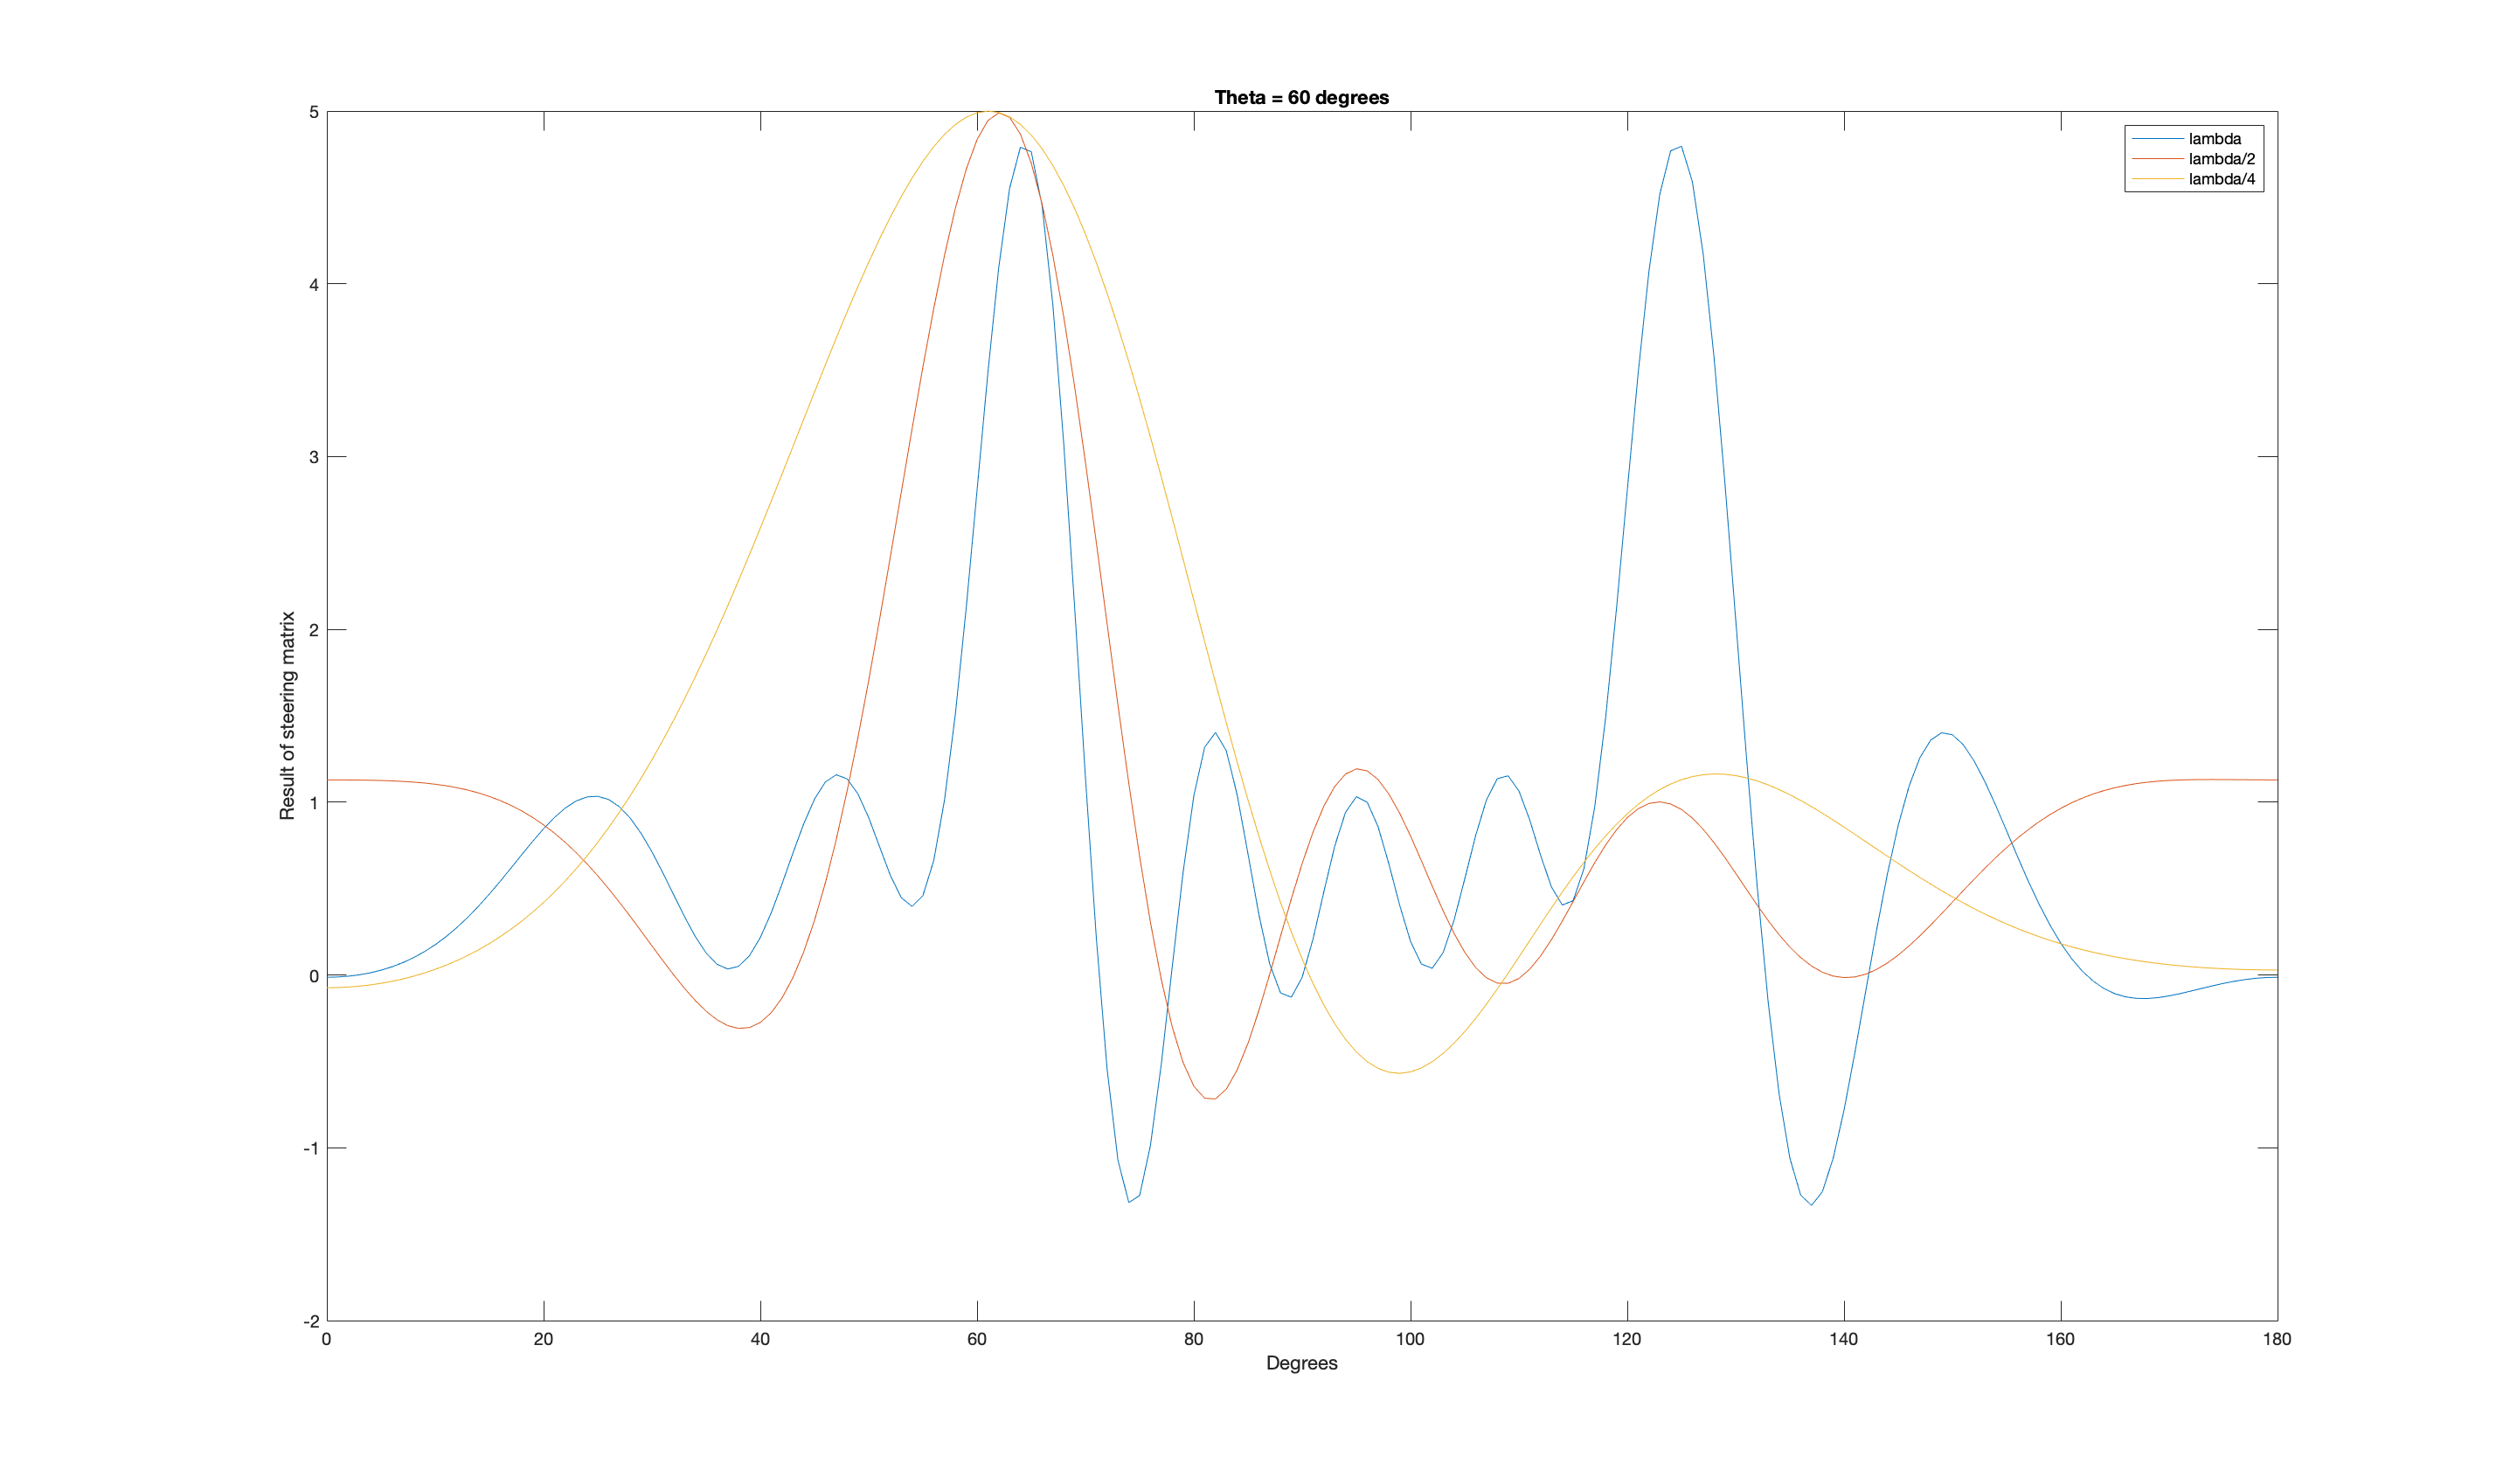
\includegraphics[width=\textwidth]{60.png}
\caption{Theta = 60 degree}
\end{figure}

b. With noise, the peak widens and becomes less sharp.

\begin{figure}[H]
\centering
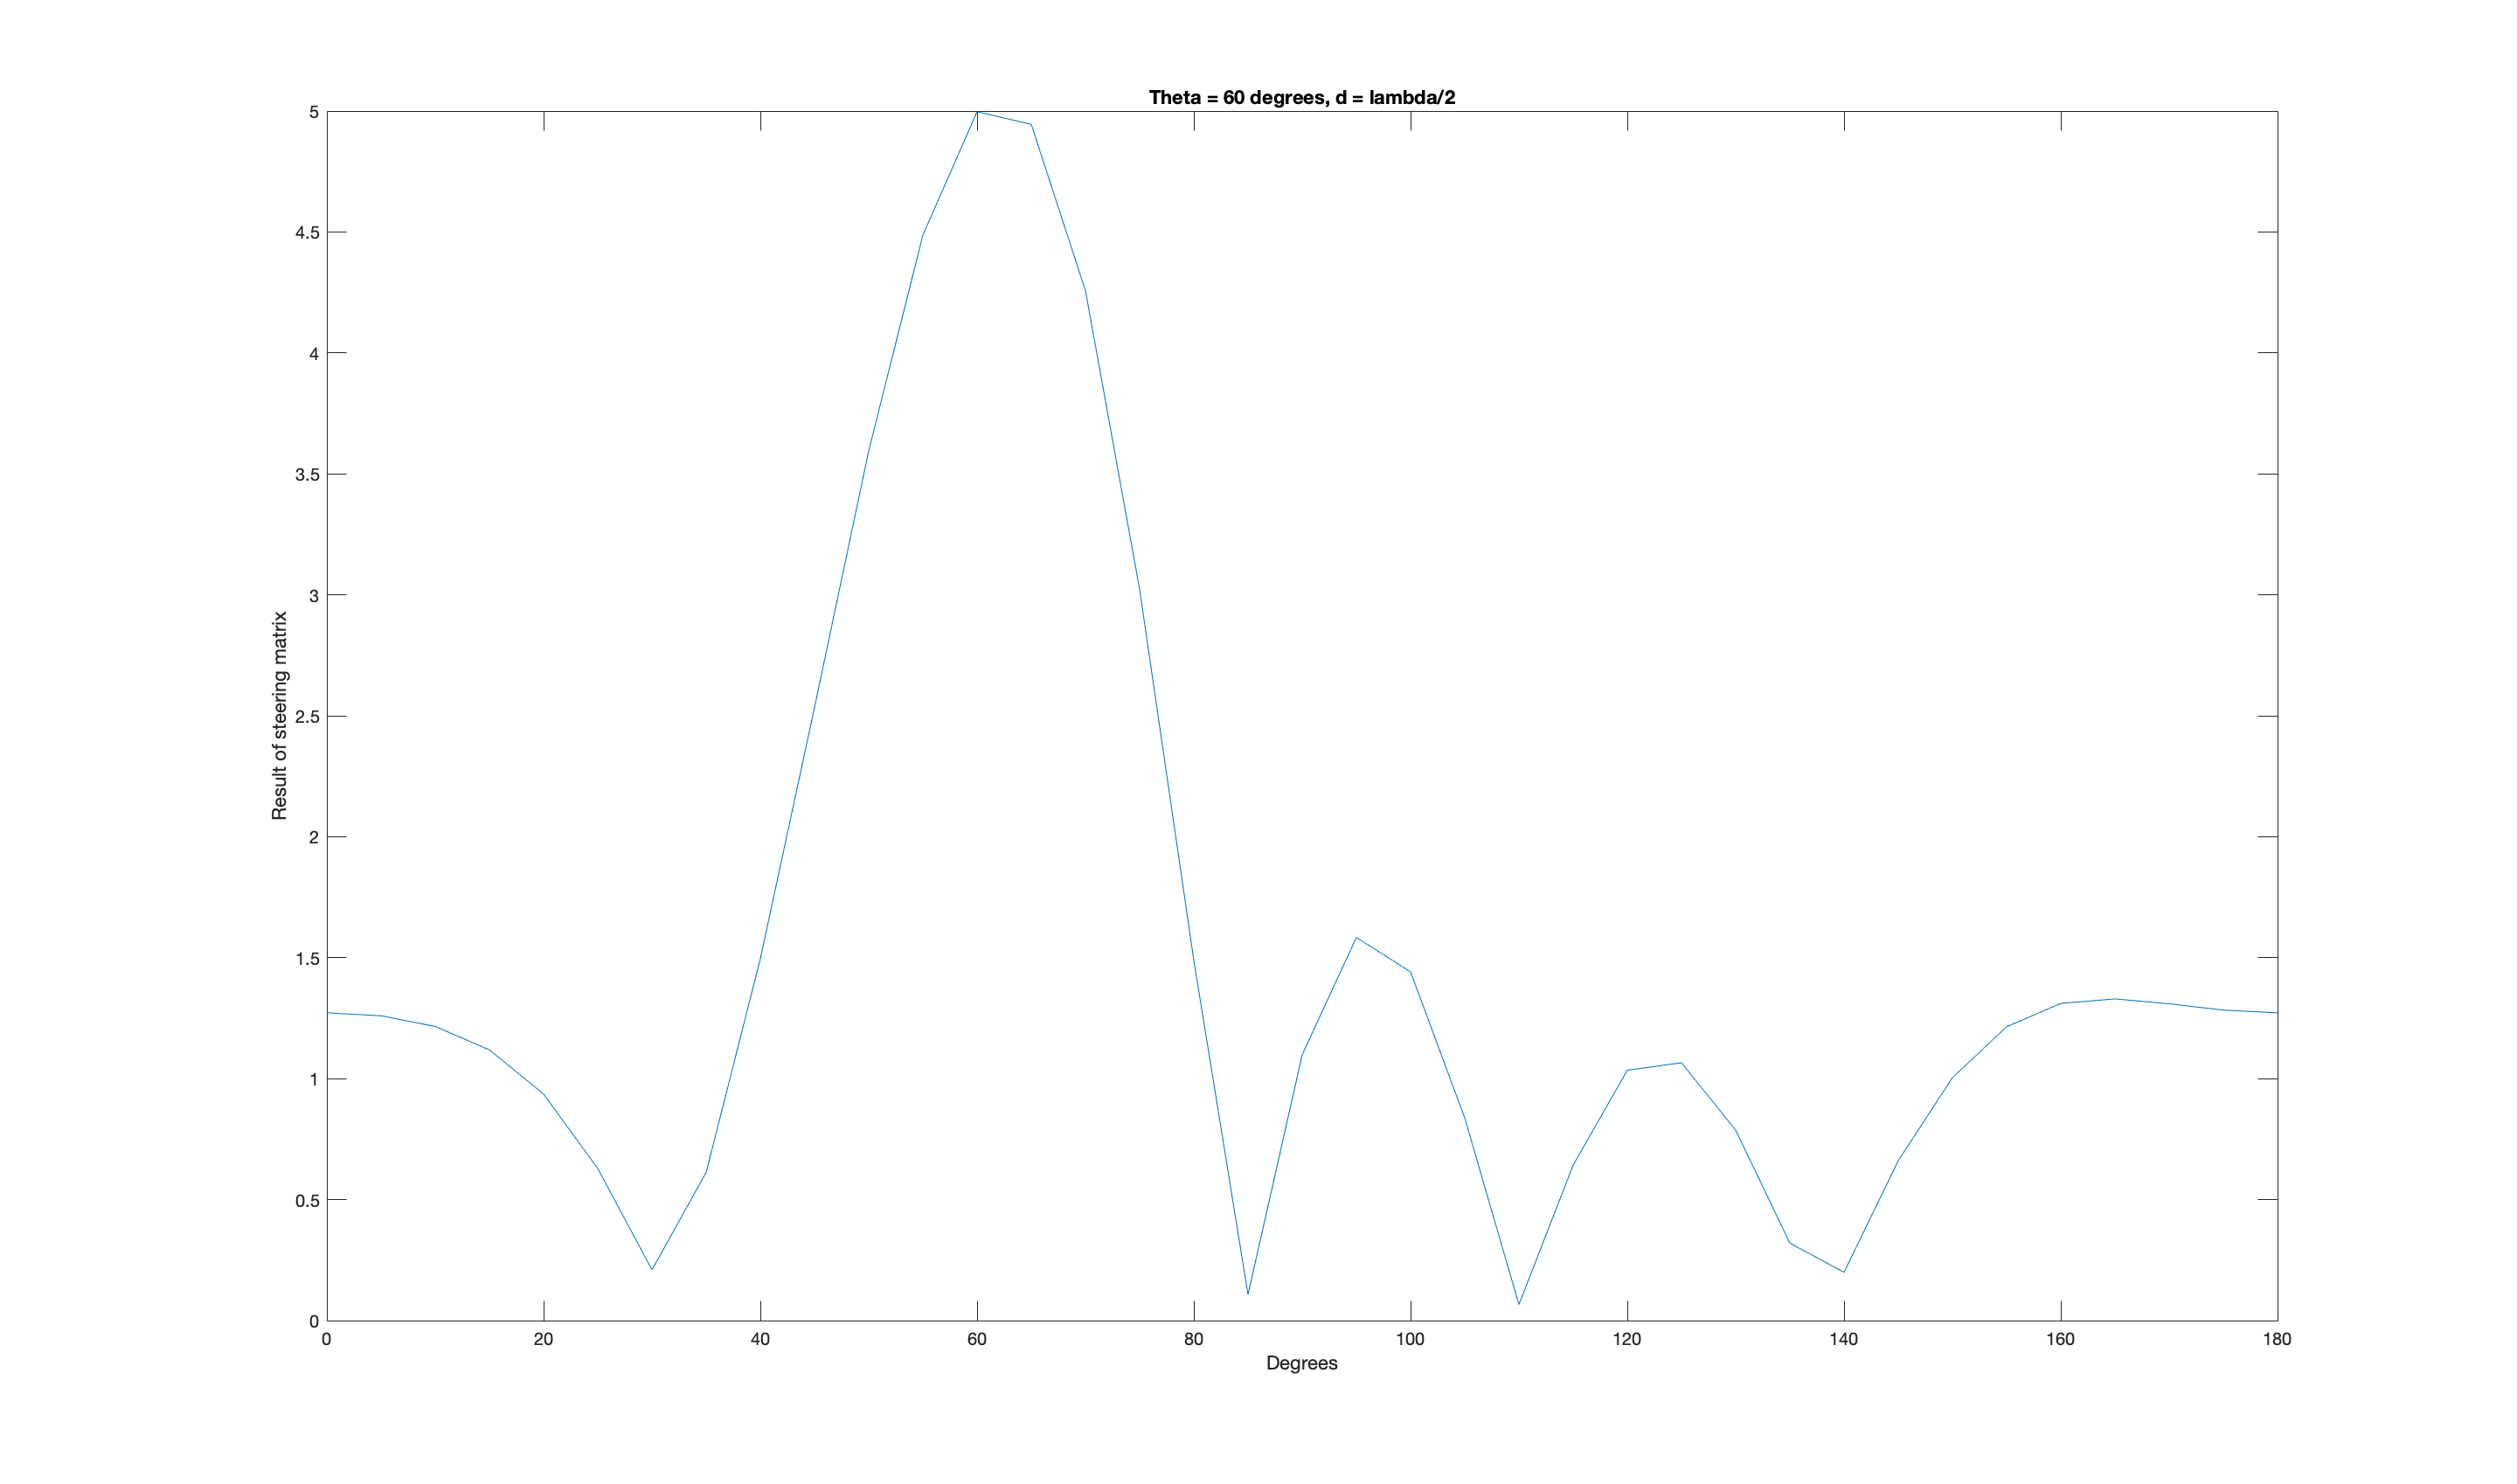
\includegraphics[width=\textwidth]{b.png}
\caption{Theta = 60 degree, d = lambda/2}
\end{figure}


c. Adding reflection path, theta = 30 and alpha = 80, d = lambda/2. Still able to detect both.

\begin{figure}[H]
\centering
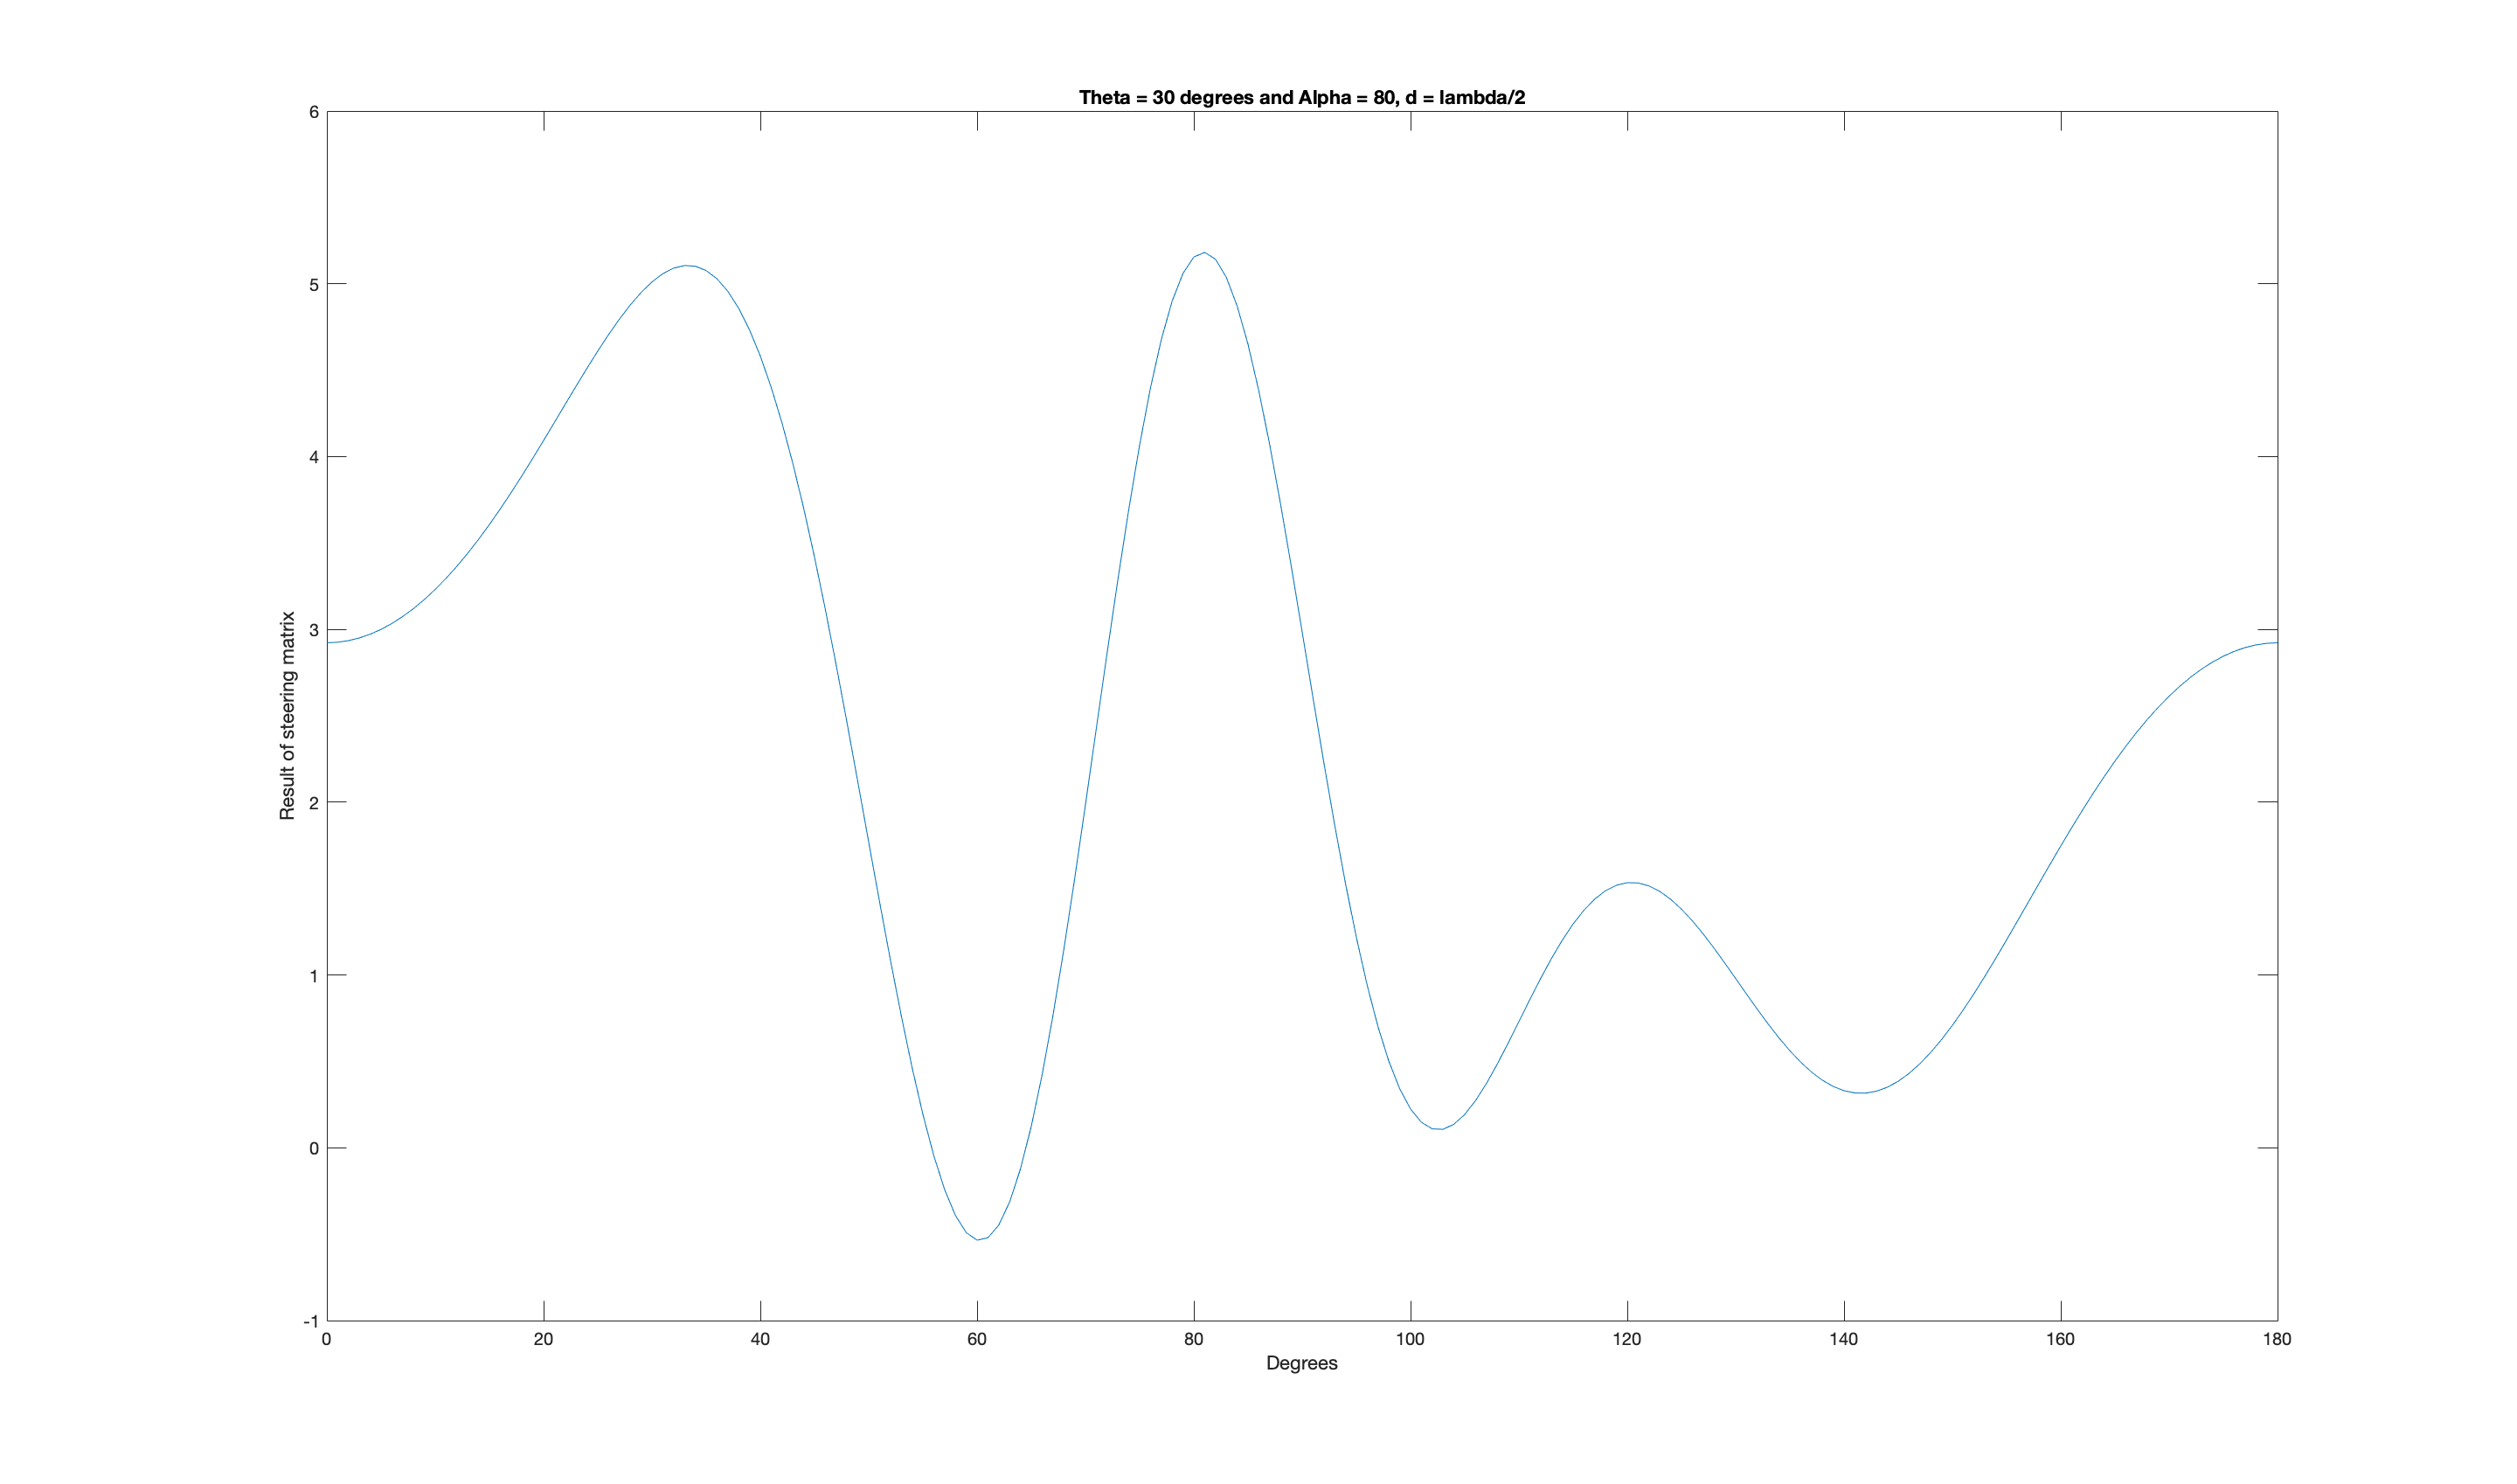
\includegraphics[width=\textwidth]{c.png}
\caption{Theta = 30 degree, Alpha = 80, d = lambda/2}
\end{figure}


d. It stops working at four reflections = [20, 66.67, 133.66, 160]. Detects 20 and 160. There are peaks around 66 and 133 as well but not accurate. A higher peak at 90 exists. 

\begin{figure}[H]
\centering
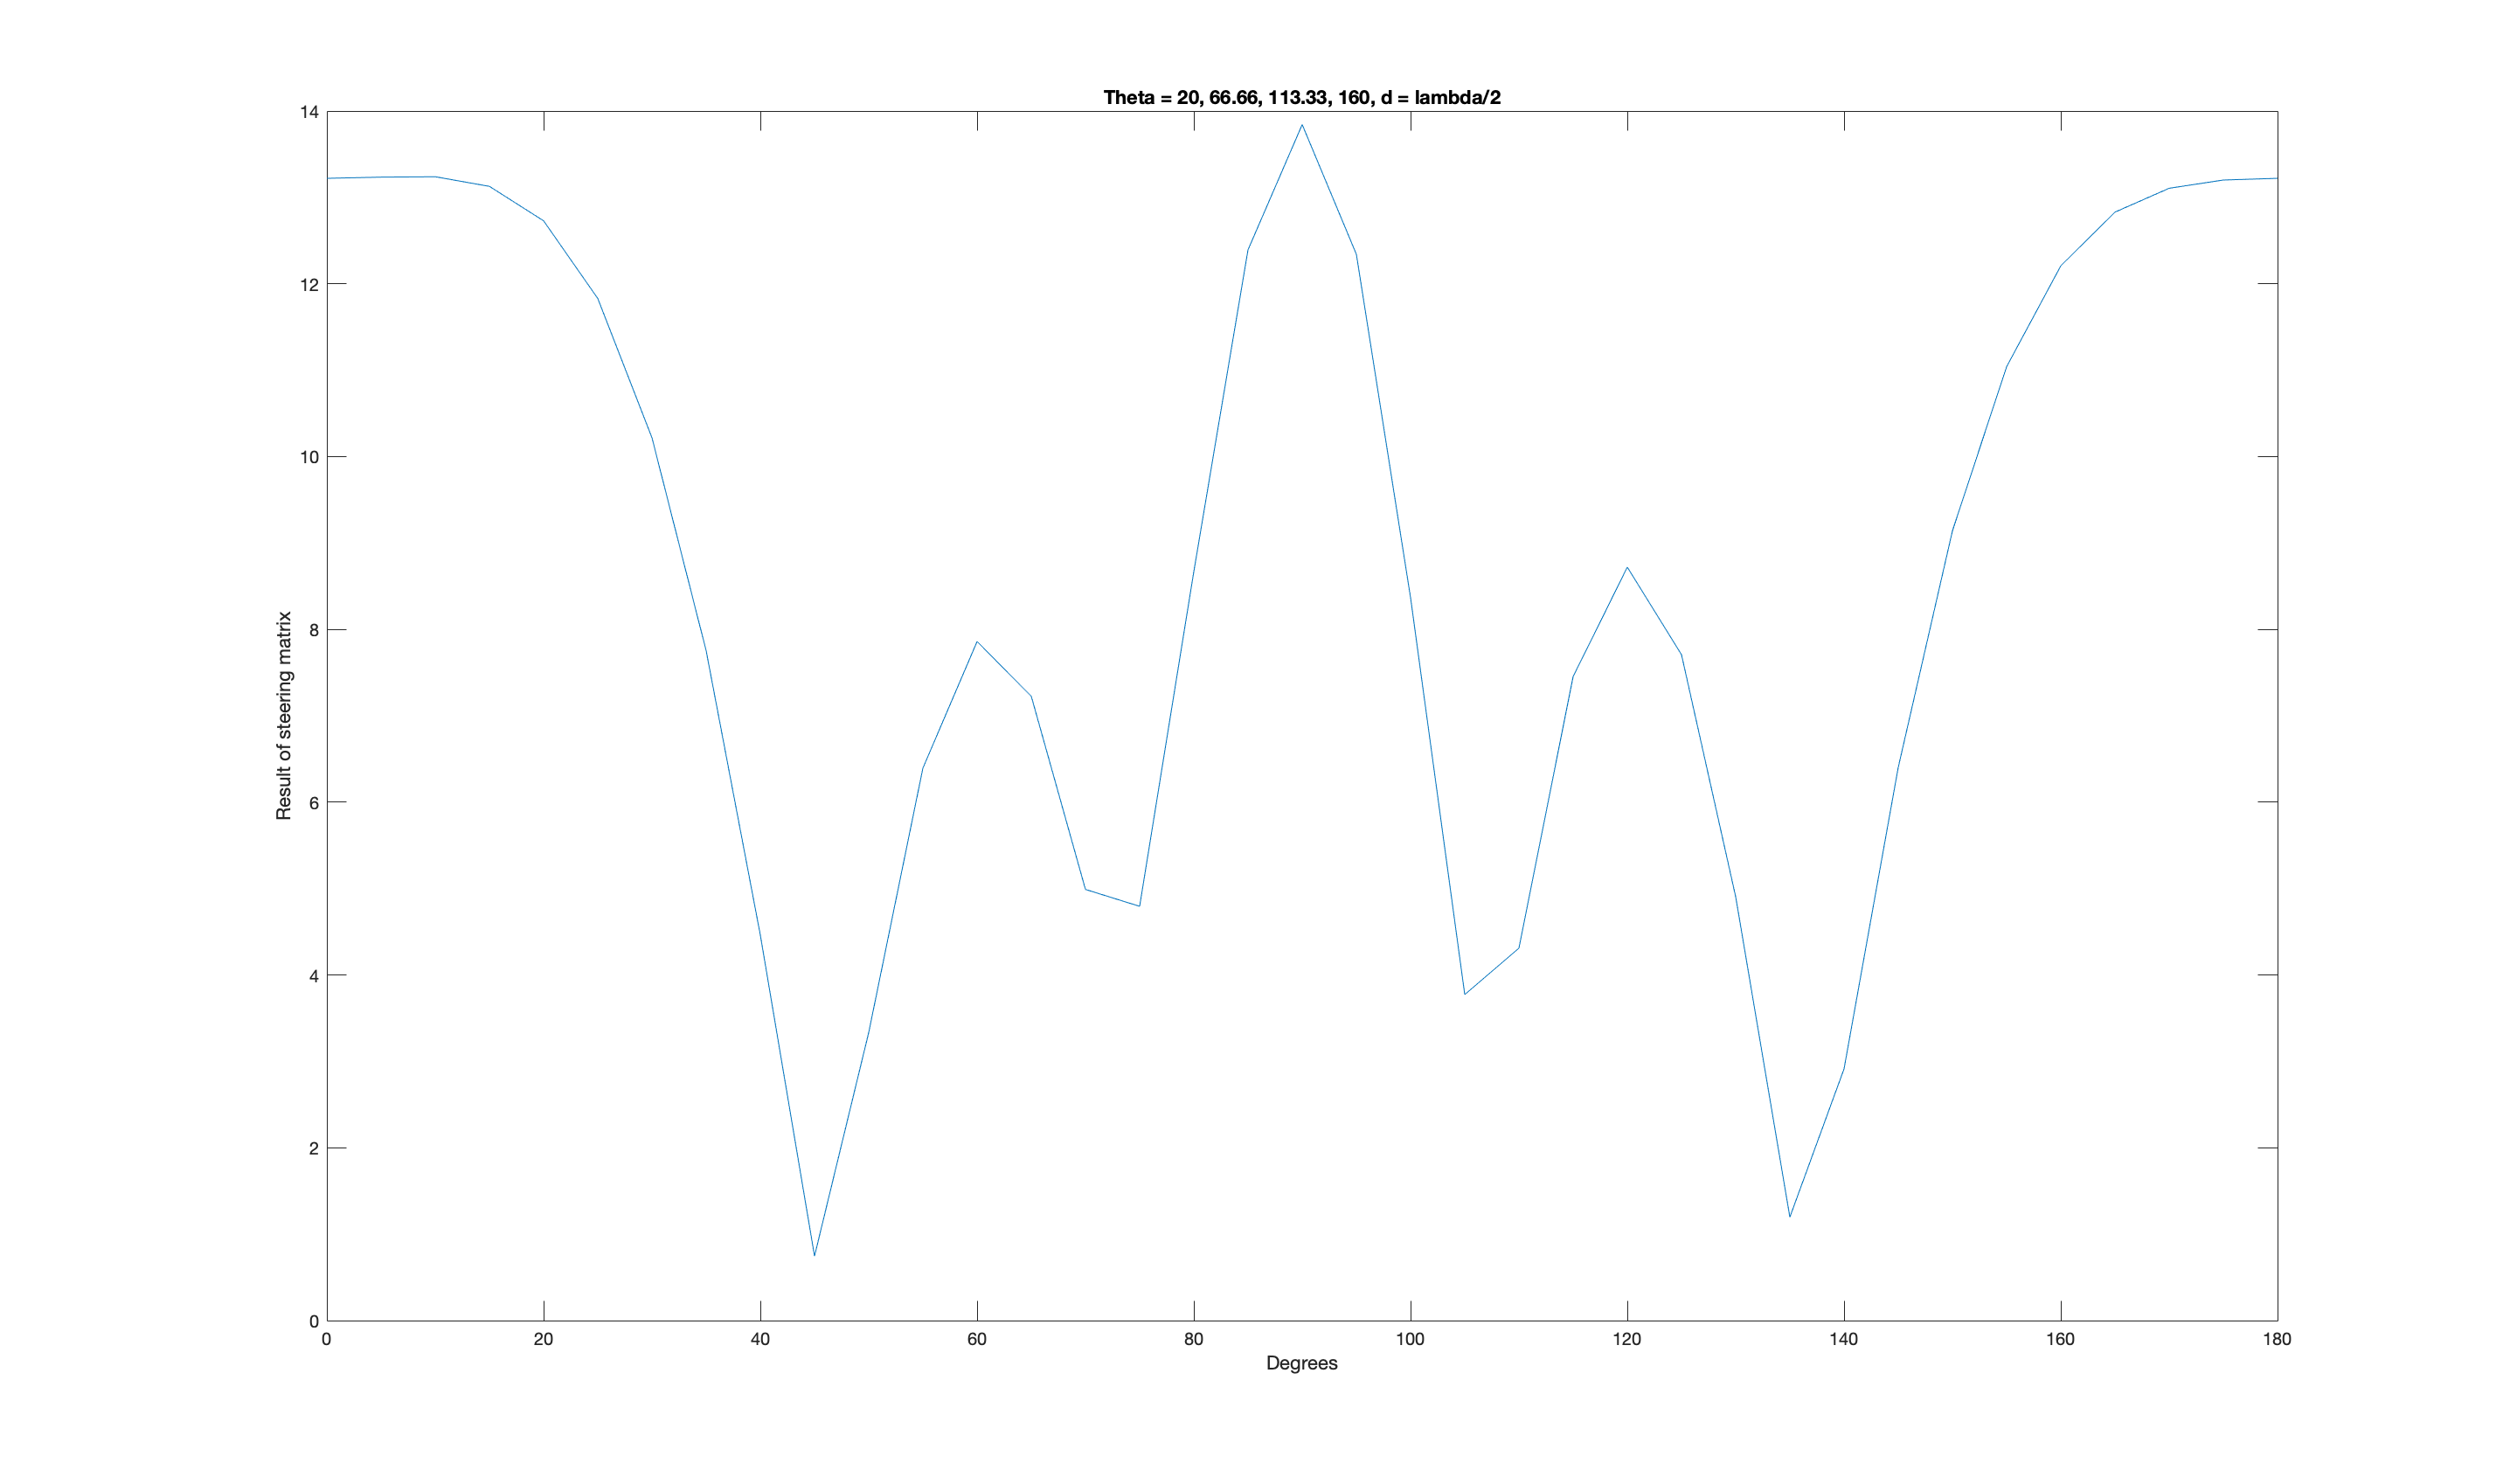
\includegraphics[width=\textwidth]{d.png}
\caption{Theta = 20, 66.67, 133.66, 160, d = lambda/2}
\end{figure}




 








%%%%%%%%%%%%%%%%%%%%%%%%%%%%%%%%%%%%%%%%%%%%%%%%%%%%%%%%%%%%%%%%%%%%%%%%%%%%%%%%%%%%%%%%%%%%%%%%%%%%%%
 


\end{document}